This test problem is a 1-D problem with a source in the left half of an
absorber and a zero incident flux imposed on the left boundary. The solution
in the left half of the domain shows the solution reaching its
saturation value $\frac{q}{\sigma}$, and the solution in the right half
is an exponential decay.
Table \ref{tab:source_in_absorber} summarizes the test parameters.

%-------------------------------------------------------------------------------
\begin{table}[htb]\caption{Source-in-Absorber Test Problem Summary}
\label{tab:source_in_absorber}
\centering
\begin{tabular}{l l}\toprule
\emph{Parameter} & \emph{Value}\\\midrule
Domain & $\mathcal{D} = (0,1)$\\
Initial Conditions & $u_0(x)=0$\\
Boundary Conditions & $u(0,t)=u_{inc}=0$\\
Direction & $\mathbf{\Omega} = \mathbf{e}_x$\\
Cross Section & $\sigma(\x)=\left\{\begin{array}{c l}
   \sigma_0, & x\in[x_0,x_1]\\
   \sigma_1, & x\in(x_1,x_2]
   \end{array}\right.,\quad
   \left[\begin{array}{c}\sigma_0\\\sigma_1\end{array}\right] =
      \left[\begin{array}{c}100\\100\end{array}\right]$\\
   & $\left[\begin{array}{c}x_0\\x_1\\x_2\end{array}\right] =
      \left[\begin{array}{c}0\\0.5\\1\end{array}\right]$\\
Source & $q(\x,t)=\left\{\begin{array}{c l}
   q_0, & x\in[x_0,x_1]\\
   q_1, & x\in(x_1,x_2]
   \end{array}\right.,\quad
   \left[\begin{array}{c}q_0\\q_1\end{array}\right] =
      \left[\begin{array}{c}10\\0\end{array}\right]$\\
Speed & $\speed=1$\\
Exact Solution & (Equation \eqref{eq:multiregion_exactsolution})\\
\bottomrule\end{tabular}
\end{table}
%-------------------------------------------------------------------------------

Table \ref{tab:source_in_absorber_run_parameters} shows the run parameters used
for the results in this section.
Figures \ref{fig:source_in_absorber_strong1},
\ref{fig:source_in_absorber_strong0},
\ref{fig:source_in_absorber_weak}, and
\ref{fig:source_in_absorber_penalty}
compares the solutions computed for each scheme using different
boundary conditions, respectively the following:
strongly imposing with $L_i^-=L_i^+=1$ for Dirichlet nodes, 
strongly imposing with $L_i^-=L_i^+=0$ for Dirichlet nodes, 
weakly imposing, and
weakly imposing with boundary penalty ($\alpha_i = 1000$).
One can see clearly from a comparison of the FCT solutions with strongly
imposed BC that cancellation of the antidiffusive fluxes from the boundary
has a significant impact on the solution; the approach to the first saturation 
value roughly follows the low-order solution because the first antidiffusive
flux was canceled. Allowing nonzero antidiffusive fluxes from the Dirichlet
node shows superior results in this case - the FCT solution follows the
high-order solution on the
first approach to saturation, which is within the FCT solution bounds. These
results illustrate a typical dilemma with this issue; accepting some antidiffusion
from a Dirichlet node does not satisfy conservation statements, but often
in practice, cancellation of antidiffusive fluxes from these nodes leads to
an inaccurate solution in the vicinity.
Weak imposition of BC here gives very inaccurate boundary values;
however, with a penalty applied, the solutions are much more accurate,
and in addition, the solution is conservative, unlike when strongly imposing
the BC with $L_i^-=L_i^+=1$ for Dirichlet nodes.

%-------------------------------------------------------------------------------
\begin{table}[ht]\caption{Source-in-Absorber Test Problem Run Parameters}
\label{tab:source_in_absorber_run_parameters}
\centering
\begin{tabular}{l l}\toprule
\emph{Parameter} & \emph{Value}\\\midrule
Number of Cells & $N_{cell} = 32$\\
Time Discretization & Steady-State\\
Boundary Conditions & (varies by run)\\\midrule
Entropy Function & $\entropy(u) = \frac{1}{2}u^2$\\
Entropy Residual Coefficient & $\entropyresidualcoef = 0.1$\\
Entropy Jump Coefficient & $\entropyjumpcoef = 0.1$\\\midrule
FCT Solution Bounds & Analytic\\
\bottomrule\end{tabular}
\end{table}
%-------------------------------------------------------------------------------
%-------------------------------------------------------------------------------
\begin{figure}[ht]
   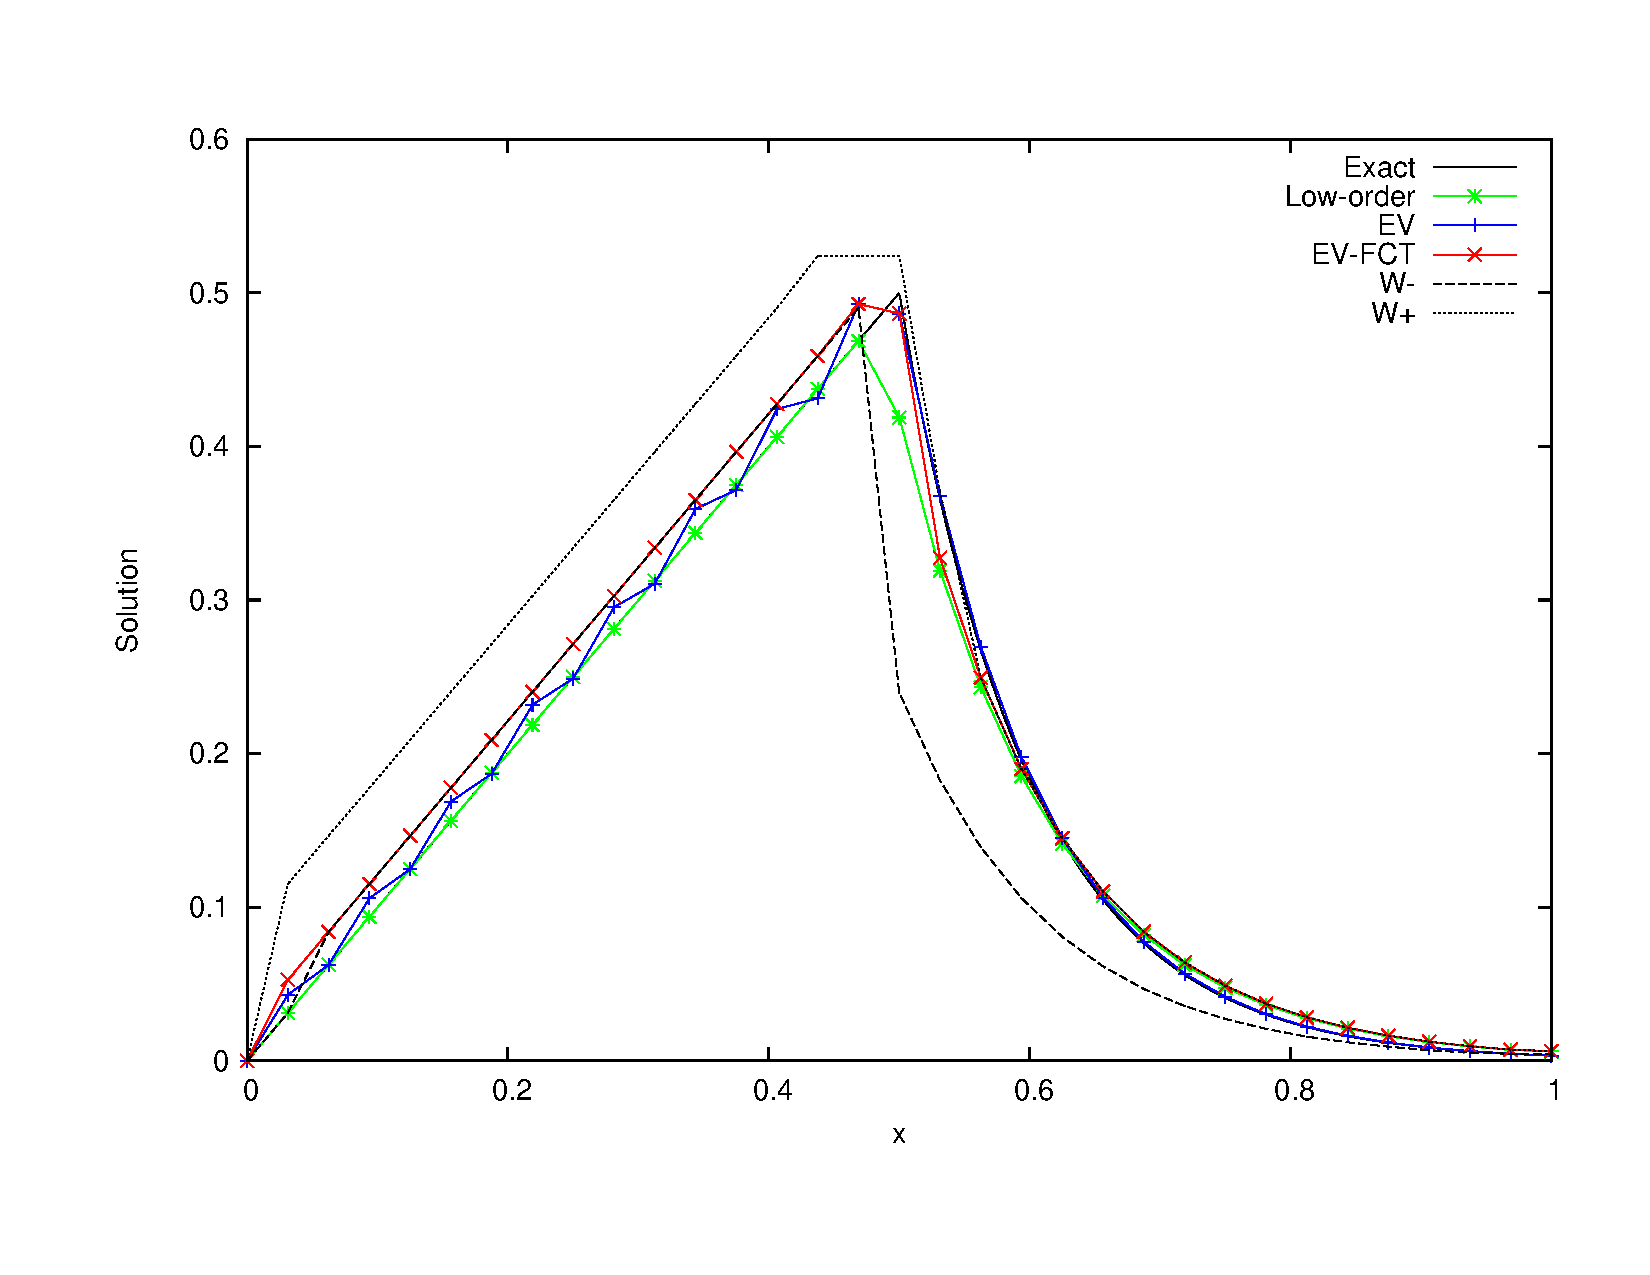
\includegraphics[width=\textwidth]
     {\contentdir/results/transport/source_in_absorber/images/strong1.pdf}
   \caption{Steady-State Solutions for the Source-in-Absorber Problem
     with Strongly Imposed Dirichlet Boundary Conditions with $L_i^-=L_i^+=1$}
   \label{fig:source_in_absorber_strong1}
\end{figure}
%-------------------------------------------------------------------------------
%-------------------------------------------------------------------------------
\begin{figure}[ht]
   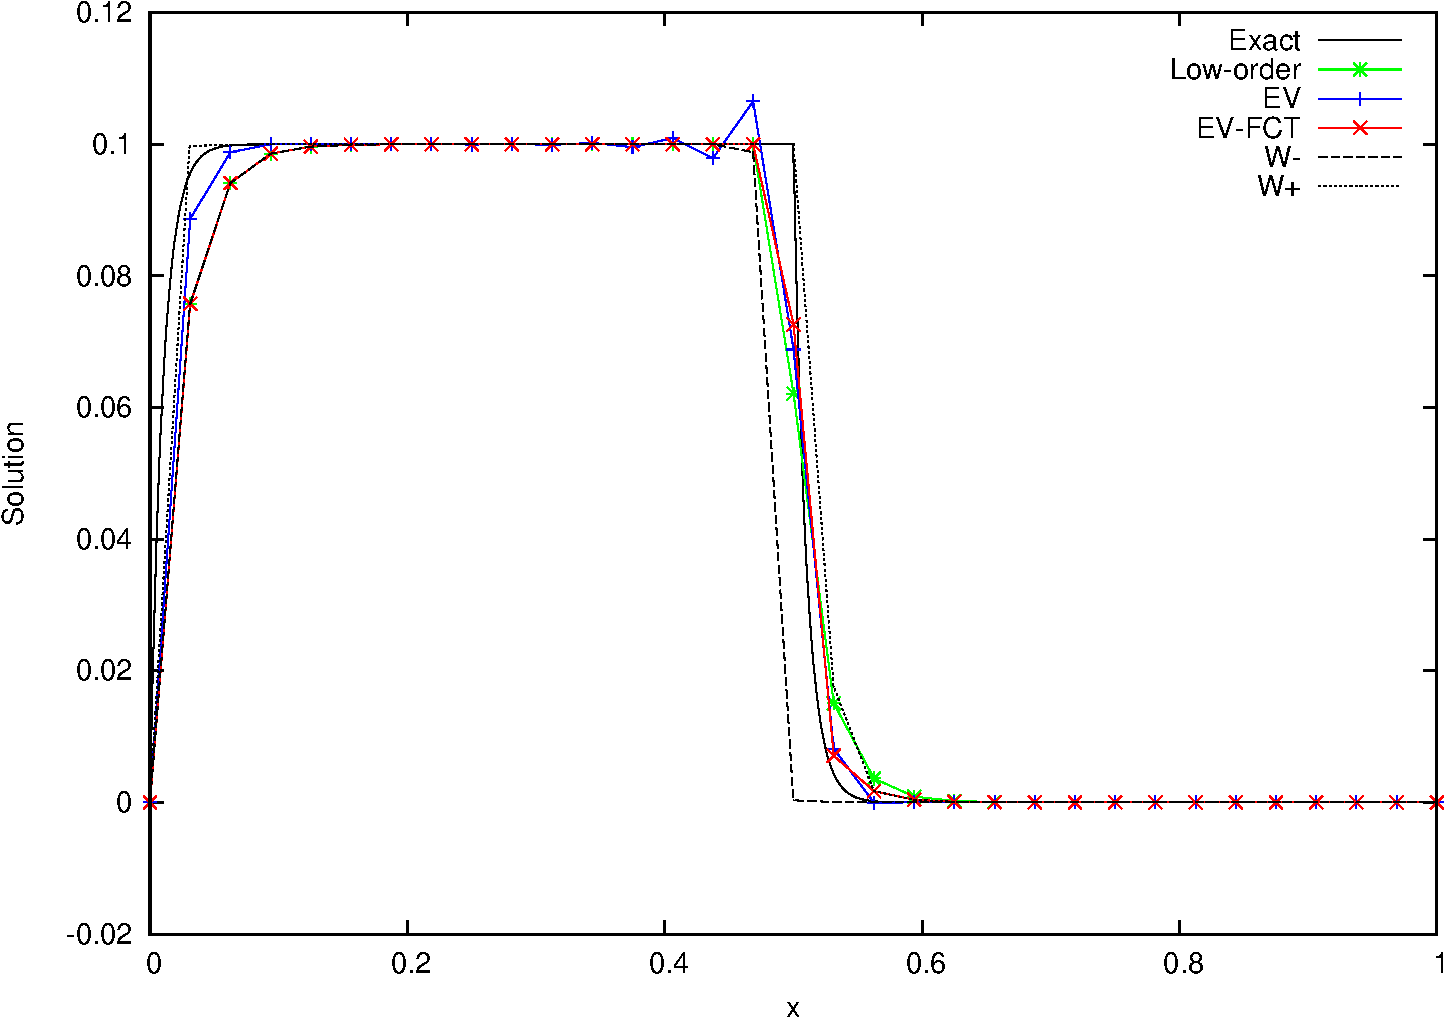
\includegraphics[width=\textwidth]
     {\contentdir/results/transport/source_in_absorber/images/strong0.pdf}
   \caption{Steady-State Solutions for the Source-in-Absorber Problem
     with Strongly Imposed Dirichlet Boundary Conditions with $L_i^-=L_i^+=0$}
   \label{fig:source_in_absorber_strong0}
\end{figure}
%-------------------------------------------------------------------------------
%-------------------------------------------------------------------------------
\begin{figure}[ht]
   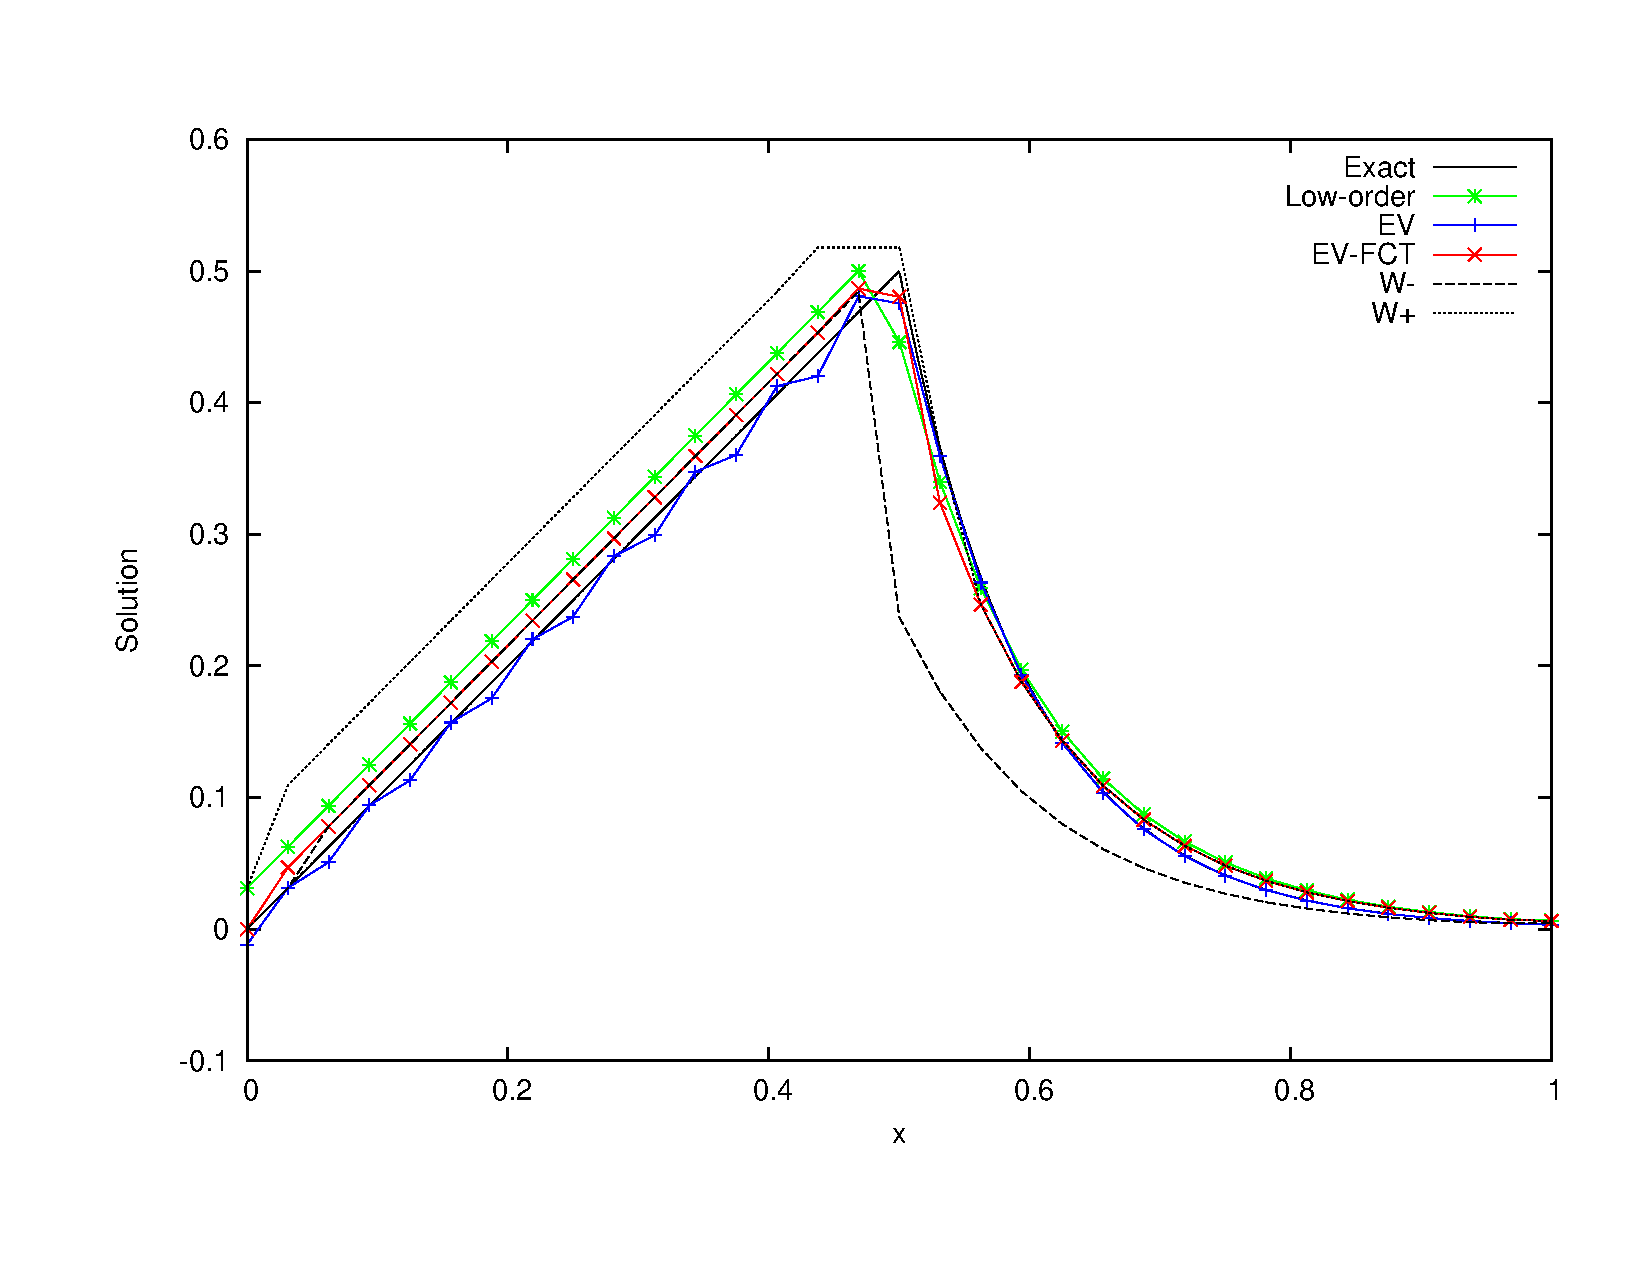
\includegraphics[width=\textwidth]
     {\contentdir/results/transport/source_in_absorber/images/weak.pdf}
   \caption{Steady-State Solutions for the Source-in-Absorber Problem
     with Weakly Imposed Dirichlet Boundary Conditions}
   \label{fig:source_in_absorber_weak}
\end{figure}
%-------------------------------------------------------------------------------
%-------------------------------------------------------------------------------
\begin{figure}[ht]
   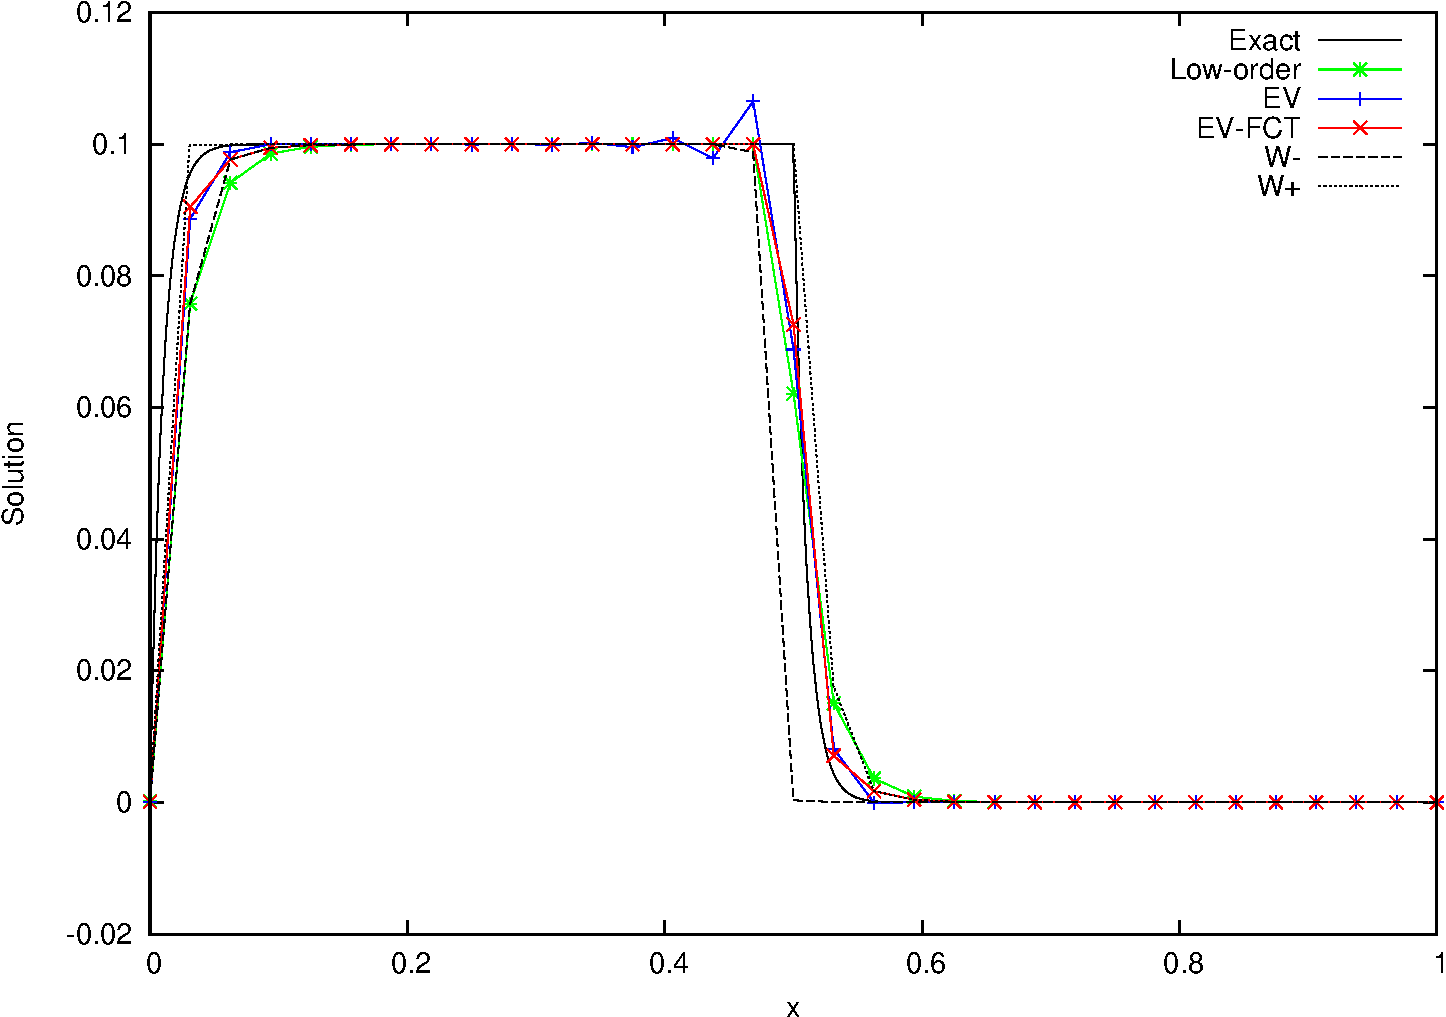
\includegraphics[width=\textwidth]
     {\contentdir/results/transport/source_in_absorber/images/penalty.pdf}
   \caption{Steady-State Solutions for the Source-in-Absorber Problem
     with Weakly Imposed Dirichlet Boundary Conditions and Boundary Penalty}
   \label{fig:source_in_absorber_penalty}
\end{figure}
%-------------------------------------------------------------------------------

\clearpage
